\documentclass{beamer}
 
\usetheme{Madrid}
\usepackage{graphicx}
\graphicspath{ {./images/} }

\title{Predicting Personality and Traits Using Machine Learning}
\subtitle{Senior Capstone I IT415 - 01}
\date{Spring 2020 2/6/20}
\author{Dustin Powell}
\institute{Cumberland University}

\begin{document}

\newtheorem{q1}{Question 1}
\newtheorem{q2}{Question 2}
 
\frame{\titlepage}

 %------------------------------------------------------------------------------
\begin{frame}
\frametitle{Introduction}
\begin{itemize}
    \item Personal data about people can be acquired from many sources.
    \item Much of this information is available through the internet.
    \begin{itemize}
        \item Example: Social Media Post, Consumers Habits, etc.
    \end{itemize}
    \item Information obtained can be used to predict other characteristics of an individual.
    \item The purpose of this work most accurately predict a person's personality and traits from this data using machine learning.
\end{itemize}
\end{frame}

 %------------------------------------------------------------------------------
\begin{frame}
\frametitle{Case Study in PNAS}
\begin{itemize}
    \item Post--liking habits of roughly 58,500 people were able to predict various private aspects about the user such as age, race, intelligence, and political views \cite{Kosinski2013}.
    \item The primary tools were used in this research were linear and logistic regression \cite{Kosinski2013}. 
    \item The users where assembled into a matrix called the User--Like matrix which shows the post that a user has liked relating to various things like products or hobbies \cite{Kosinski2013}. 
    \item Singular Value Decomposition was then used on the set of data and then assembled into a User--Components Matrix to use the linear and logistic regression to make the predictions \cite{Kosinski2013}. 
    \item  The study has raised numerous ethical questions as well such as what would happen if the wrong person found out this information  \cite{Kosinski2013}.
\end{itemize}
\end{frame}

%------------------------------------------------------------------------------
\begin{frame}
\frametitle{Questions to Address}
The following questions arise from the case study by Kosinski, Stillwell, and Graepel \cite{Kosinski2013}
\begin{q1}
Using a machine learning algorithm what is the minimum amount of information needed to predict the traits and personality of a given person accurately? 
\end{q1}
\begin{q2}
Can a person protect their private information about themselves?
\end{q2}
\end{frame}

%------------------------------------------------------------------------------
\begin{frame}
\frametitle{Relationship Between Big Data and Predictive Analytics}
\begin{itemize}
    \item The previous case study is a specific example of a much larger and increasely important field. 
    \item Big Data is the concept of collecting information from various online sources to be processed and or stored in databases to be used \cite{Jeble2016}.
    \item Three types of data that are collected \cite{Jeble2016}:.
    \begin{itemize}
    \item Structured
        \begin{itemize}
        \item Example: Sales Figures
        \end{itemize}
    \item Unstructured
        \begin{itemize}
        \item Example: Social Media Posts
        \end{itemize}
    \item Semi--Structured
        \begin{itemize}
        \item Example: SQL Scripts, Server Logs
        \end{itemize}
    \end{itemize}
\item Unstructured and semi--structured data have to be processed before storage versus structured that can be immediately stored into a database \cite{Jeble2016}.
\end{itemize}
\end{frame}

%------------------------------------------------------------------------------
\begin{frame}
\frametitle{Forms of Analytics}
\begin{itemize}
    \item Three forms of analytics that are performed on the data stored in databases \cite{Jeble2016}.
    \begin{itemize}
    \item Descriptive Analytics
        \begin{itemize}
        \item Analysis of data past occurrences of events.
        \end{itemize}
    \item Predictive Analytics
        \begin{itemize}
        \item  Analysis of data to make predictions.
        \end{itemize}
    \item Prescriptive Analytics
        \begin{itemize}
           \item Analysis of data to make decisions.
        \end{itemize}
    \end{itemize}
    \item The application of statistics and computer science allow for these various forms of analytics to be conducted \cite{Jeble2016}.
\end{itemize}
\end{frame}

%------------------------------------------------------------------------------
\begin{frame}
\frametitle{Overview of The Relationship}
\begin{figure}
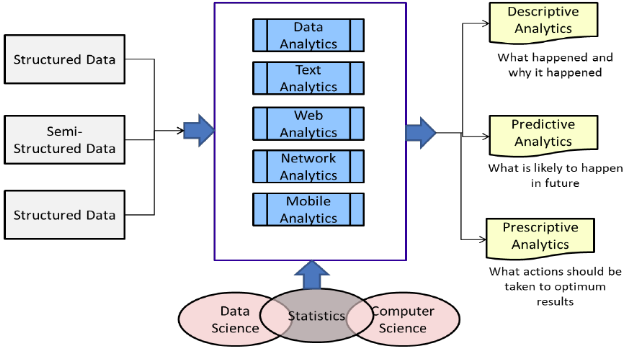
\includegraphics[scale=2]{BigDataDiagram}
\caption{Visual representation,  similar to a SQL ER--diagram, of the relationship between analytics and Big Data from the 2016 publication by Jeble, Kumari, and Patel \cite{Jeble2016}.}
\end{figure}
\end{frame}

%------------------------------------------------------------------------------
\begin{frame}
\frametitle{Use of Predictive Analytics in Business}
\begin{itemize}
    \item Analytics is used by businesses to make educated decisions by using the resource as a way to understand markets \cite{Jeble2016}.
    \item Predictive analytics can be used for predicting sales outcomes of a company's product versus the market competition \cite{Jeble2016}.
    \item Marketing uses predictive analytics to determine which ads to deliver to internet users \cite{Jeble2016}.
        \begin{itemize}
        \item Example: Youtube Video Advertisements 
        \end{itemize}
\end{itemize}

\end{frame}

%------------------------------------------------------------------------------
\begin{frame}
\frametitle{Regression and Predictive Analytics}
\begin{itemize}
    \item Linear and multiple regression in general determines possible correlations between independent and dependent variables assuming a functional relationship between them to make predictions \cite{Stats2015}. 
    \item In most cases multiple independent variables exist so multiple regression is used.
    \item Limitations in this technique are that functions must be assumed or that too many independent variables exist.
\end{itemize}
\end{frame}

%------------------------------------------------------------------------------
\begin{frame}
\frametitle{What is Machine Learning}
\begin{itemize}
\item Machine Learning is a subsection of artificial intelligence that is specifically focused on using algorithms to make conclusions about a set of information \cite{pythonML}.
%Clean up bullet structure
\item Three types of machine learning:
\item Supervised Machine Learning
    \begin{itemize}
        \item Using a base set of data to train the algorithm in which then makes predictions based on the learned information \cite{pythonML}.
    \end{itemize}
\item Unsupervised Machine Learning
    \begin{itemize}
        \item The use of an algorithm to classify and find relationships within a set of data without knowing of any results \cite{pythonML}.
    \end{itemize}
\item Reinforcement Machine Learning
    \begin{itemize}
    \item The use of a agent that learn from task carried out that results in a reward for correctly carrying out the task \cite{pythonML}.
    \end{itemize}
\end{itemize}
\end{frame}

%------------------------------------------------------------------------------
\begin{frame}
\frametitle{The Iris Data Set}
\begin{itemize}
    \item The iris data set is a classic data set of machine learning
    \item The data set is comprised of sepal and petal measurements of iris flowers\cite{IrisData}.
    \item The set of information includes three types of iris called Setosa, Versicolor, and Virginica  \cite{IrisData}.
    \item Each of the flower has their sepal and petal width and length taken as the identify features of the flower  \cite{IrisData}.
    \item The data set was created by R. A. Fisher in 1936 for the purpose of pattern recognition  \cite{IrisData}.
\end{itemize}
\end{frame}

%------------------------------------------------------------------------------
\begin{frame}[fragile]
\frametitle{Example of Mahcine Learning Algorithm Using Iris Data Set}
\fontsize{6}{5}
\begin{verbatim}
# make predictions
from pandas import read_csv
from sklearn.model_selection import train_test_split
from sklearn.metrics import classification_report
from sklearn.metrics import confusion_matrix
from sklearn.metrics import accuracy_score
from sklearn.svm import SVC

def main():
    # Load dataset
    csvData = "iris.csv"
    names = ['sepal-length', 'sepal-width', 'petal-length', 'petal-width', 'class']
    dataset = read_csv(csvData, names=names)
    # Split-out validation dataset
    array = dataset.values
    X = array[:,0:4]
    y = array[:,4]
    X_train, X_validation, Y_train, Y_validation = train_test_split(X, y, test_size=0.20, random_state=1)
    # Make predictions on validation dataset
    model = SVC(gamma='auto')
    model.fit(X_train, Y_train)
    predictions = model.predict(X_validation)
    # Evaluate predictions
    print(accuracy_score(Y_validation, predictions))
    print(confusion_matrix(Y_validation, predictions))
    print(classification_report(Y_validation, predictions))

main()
\end{verbatim}
The algorithm is made by Brownlee to teach people about machine learning with slight edits to load to load a CSV file from the computer \cite{MLAlg}.
\end{frame}

%------------------------------------------------------------------------------
\begin{frame}[fragile]
\frametitle{Sample Algorithm Output}
Below is the sample output from running the algorithm:
\begin{verbatim}
0.966666666667
[[11  0  0]
 [ 0 12  1]
 [ 0  0  6]]
                 precision    recall  f1-score   support

    Iris-setosa       1.00      1.00      1.00        11
Iris-versicolor       1.00      0.92      0.96        13
 Iris-virginica       0.86      1.00      0.92         6

    avg / total       0.97      0.97      0.97        30

\end{verbatim}
\end{frame}

%------------------------------------------------------------------------------
\begin{frame}
\frametitle{Objectives to Accomplish}
A brief overview of the upcoming objectives to accomplish.
\begin{enumerate}
     \item Further defining and explanation of terminology and topics of machine learning
     \item Locate a data set(s) of people's traits 
     \item Design a program using python to predict a person's traits
     \item Test to determine if correct results about a person can be made.
     \item Answer Question Two: Privacy?
     \item Explain and adding additional details as needed.
\end{enumerate}
\end{frame}

%------------------------------------------------------------------------------
\begin{frame}
\frametitle{References}
\fontsize{9}{11}
\begin{thebibliography}{9}

\bibitem[1]{Kosinski2013}
M. Kosinski, D. Stillwell, and T. Graepel (2013),
''Private traits and attributes are predicatable from digital records of human behavior'', \textit{PNAS} 110. 15. , 5802 - 5805. Google Scholar. Accessed January 19th 2020 URL:https://www.pnas.org/content/pnas/110/15/5802.full.pdf

\bibitem[2]{Stats2015}
J. Bothe, J. L. Brudney, and K. J. Meier (2015), \textit{Applied Statistics For Public and Nonprofit Administration}. 4th ed. Stamford, CT USA Cengage Learning.

\bibitem[3]{Jeble2016}
S. Jeble, S. Kumari, and Y. Patil (2016),
''Role of big data and predictive analytics''. \textit{International Journal of Automation and Logistics}. 2. 307-331. 10.1504/IJAL.2016.10001272. Google Scholar. Accessed January 21st 2020 URL: https://www.researchgate.net/publication/309809606

\bibitem[4]{pythonML}
V. Mirjalili and S. Raschka (2017),
\textit{Python Machine Learning}. 2nd ed. Birmingham, UK Packt Publishing.

\bibitem[5]{IrisData}
"Iris Data Set'', University of California Irvine Machine Learning Repository. Accessed February 5th 2020 URL: https://archive.ics.uci.edu/ml/datasets/iris

\bibitem[6]{MLAlg}
J. Brownlee (2019),
''Your First Machine Leaning Project in Python Step--By--Step'', Machine Learning Mastery. Accessed February 5ht 2020. URL: https://machinelearningmastery.com/machine-learning-in-python-step-by-step/

\end{thebibliography}
\end{frame}
 
\end{document}